\chapter{Análise Bibliográfica sobre Sistemas de Recomendação de Notícias, por Tatiana Franco Pereira\label{chap:bibliometria:Tatianafp}}

\section{Planejamento do estudo}

Após a transposição do conteúdo dos jornais impressos para o formato digital, sites e aplicativos de notícias passaram a ser fonte de um conteúdo gigantesco de informações, que é distribuído ao longo de inúmeras páginas. Com isso, a navegação do usuário durante o seu consumo de informação se tornou mais complexa, ao mesmo tempo em que sua navegação pelo conteúdo apresentado tem o potencial de se tornar mais personalizado. Sistemas de recomendação de notícias tem por objetivo manter o usuário interessado no conteúdo que lhe é ofertado no site ou aplicativo de notícias, com usuário mais engajados e uma maior navegação em suas páginas, a fonte de informação ganha maior relevância, além de arrecadar mais dinheiro por meio de campanhas e marketing para outras empresas. 

Tendo isso em vista, este trabalho teve por objetivo responder as seguintes perguntas:
\begin{itemize}
    \item Qual a base de conhecimentos científicos produzida em torno do tema sistemas de recomendação de notícias? 
    \item Quais os principais termos e conceitos ligados à frente de pesquisa no tema sistemas de recomendação de notícias? 
    \item Qual a estrutura social da comunidade, se é que existe, que pesquisa sobre o tema sistemas de recomendação de notícias?
    \item Quanto o Brasil estaá inserido na comunidade de pesquisadores do tema sistemas de recomendação de notícias? 
\end{itemize}

\subsection{Uso do Bibliometrix e Biblioshiny}

Para este estudo, serão utilizadas as ferramentas Bibliometrix e Biblioshiny, executadas por meio do RStudio.

\subsection{Limitações} 

O exercício foi feito em uma semana, envolvendo aproximadamente 7 horas de trabalho, utilizando a base de dados Web of Science (WoS).

\section{Coleta de dados}

A coleta de dados feita usando o WoS no dia 07 de fevereiro de 2022, acessado por meio do Portal de Periódicos da CAPES.

Foram feitas buscas nas coleções \textbf{Science Citation Index Expanded (SCI-EXPANDED), Social Sciences Citation Index (SSCI), Conference Proceedings Citation Index – Science (CPCI-S), Emerging Sources Citation Index (ESCI)}, que contém registros relativos a vários campos do conhecimento. Os artigos nessas duas coleções são indexados desde 1945. 

\subsection{Query de Busca}

Foi usada a \textit{query} de busca ilustrada na listagem:

\lstinputlisting[numbers=left,basicstyle=\normalsize\ttfamily,caption={Query de busca sobre Sistemas de Recomendação de Notícias.}]
{experiments/Tatianafp/PesquisaBibliometrica/query.txt}

\subsubsection{Explicação para os termos de busca usados\label{MASSA:query}}

A busca consistiu de duas cláusulas unidas por uma conjunção \textit{and}. A primeira foi aplicada à busca por tópico, ou seja, o termo de busca poderia aparecer no Título, no Abstract, na Author Keywords, ou nas Keywords Plus da referência. Já a segunda foi aplicada à busca por categorias. 

O termo \texttt{news recommendation systems} foi usados na primeira cláusula da \query\  para recuperar artigos que tenham em seu título, palavras-chave e resumo, termos relacionados a sistemas de recomendação de notícias. Foi usado um único termo devido à forte adesão ao termo por parte dos pesquisadores desta área.

A busca foi limitada às categorias \texttt{ Computer Science Information Systems}, \texttt{ Computer Science Artificial Intelligence} e \texttt{Computer Science Interdisciplinary Applications} por meio da segunda cláusula, visando concentrar os resultados da pesquisa à trabalhos relacionados às áreas de Sistemas de Informação, Inteligência Artificial e Aplicações Interdisciplinares. 

\subsection{Registros recuperados}

Os 452 registros obtidos como resultado da busca encontram-se em \url{https://www.webofscience.com/wos/woscc/summary/a921d816-49be-44eb-94ec-d0430ce03243-22c82fa6/relevance/1}. 

Foram utilizadas as opções \textit{Exportar registros para arquivo Bibtex} e \textit{Gravar Conteúdo: Registro completo e Referências citadas} no WoS, para que as citações também fosse usadas em análises da citações.

\section{Análise dos Dados}

\subsection{Filtragem de registros}

Antes da análise, foi aplicado um filtro sobre o \dataset\ inicial, que era formado por 452 registros,contendo pŕevias de artigos, artigos de conferência, entre outros. Foram removidos os registros de prévias de artigos, restando 446 registros após a filtragem. Este conjunto de artigos será chamado de NewsRec@Tatianafp. 

\subsection{Análise bibliográfica descritiva do \textit{dataset} }

Será apresentado a seguir, uma análise bibliométrica descritiva do \dataset\   NewsRec@Tatianafp, a qual visa fazer um descrição inicial do conjunto de registros. Tal análise foi gerada pela função \texttt{biblioAnalysis}.

As informações mais gerais sobre o \dataset\ NewsRec@Tatianafp são as seguintes:

\begin{description}
    \item [\textit{Timespan}]  Os artigos que atenderam aos critérios de busca e filtragem foram publicados a partir de 1994, até 2021. Ou seja, não foram encontrados registros entre 1945 e 1993.
    \item [\textit{Sources (Journals, Books, etc)}] São 311 fontes de informação que publicaram os documentos recuperados no \dataset\  NewsRec@Tatianafp. Ou seja, em média, cada \textit{scientific journal} publicou $446/311=1,43$ artigos. 
    \item [\textit{Average years from publication}] A média do tempo de publicação dos artigos no \dataset\  NewsRec@Tatianafp é de 6,37 anos.
    \item [\textit{Average citations per documents}] Cada artigo no \dataset\   NewsRec@Tatianafp  foi citado, em média 13,11 vezes.
    \item [\textit{Average citations per year per doc}] Cada artigo no \dataset\   NewsRec@Tatianafp  foi citado, em média 1,704 vezes por ano.
    \item [\textit{References}] O \dataset\  NewsRec@Tatianafp contém 10463 referências citadas.
    \item [\textit{Keywords Plus (ID)}] 193 distintas palavras-chave do tipo Keywords Plus (ID) foram encontradas no \dataset\ NewsRec@Tatianafp. 
    \item [\textit{Author's Keywords (DE)}] 1.180 distintas palavras-chave indicadas pelos autores foram encontradas no \dataset\ .
    \item [\textit{Authors}] 1.222 distintos nomes de autores foram encontrados no \dataset\ .
    \item [\textit{Author Appearances}] Os 1.528 distintos (nomes de) autores foram encontrados 23.470 vezes, como autores de artigos.
    \item [\textit{Authors of single-authored documents}] Dentre os 1.528 distintos (nomes de) autores encontrados, 24 deles editaram artigos individualmente, isso é, sem co-autores.
    \item [\textit{Authors of multi-authored documents}] Dentre os 1.528 distintos (nomes de) autores encontrados, 1.198 deles editaram artigos com um ou mais co-autores"
    \item [\textit{Single-authored documents}] Dentre os 446 documentos presentes no \dataset\   NewsRec@Tatianafp, 26 foram escritos por um único autor, e os 420 restantes foram elaborados em co-autoria.
    \item [\textit{Documents per Author}] Dentre os 1.528 distintos (nomes de) autores, cada um publicou em média 0,365 artigos.
    \item [\textit{Authors per Document}] Cada um dos 446 documentos presentes no \dataset\   NewsRec@Tatianafp foi autorado com 3,35 autores em média ($19.410 / 5.787 = 3,35$).
    \item [\textit{Co-Authors per Documents}] As 1.528 aparições de (nomes de) autores (``Author Appearances''), sem distribuem, em média 2,74 vezes para os 446 documentos do \dataset\  NewsRec@Tatianafp.
    \item [\textit{Collaboration Index}] Os 1.198 (nomes de) autores que editaram artigos com um ou mais co-autores, colaboraram em media 3,43 vezes para editar os 446 artigos elaborados em co-autoria, gerando, assim, um índice de colaboração 2,85. 
\end{description}

\subsection{Análise da Evolução da Produção Científica}

Com o Bibliometrix, podemos analisar como a produção científica de artigos sobre o tema Sistemas de Recomendação de Notícias evoluiu ao longo dos anos, segundo o \dataset\  NewsRec@Tatianafp. Ao realizar essa análise, encontramos a imagem \ref{fig:evol_anual_NewsRec_Tatianafp}. 

\begin{figure}
    \centering
    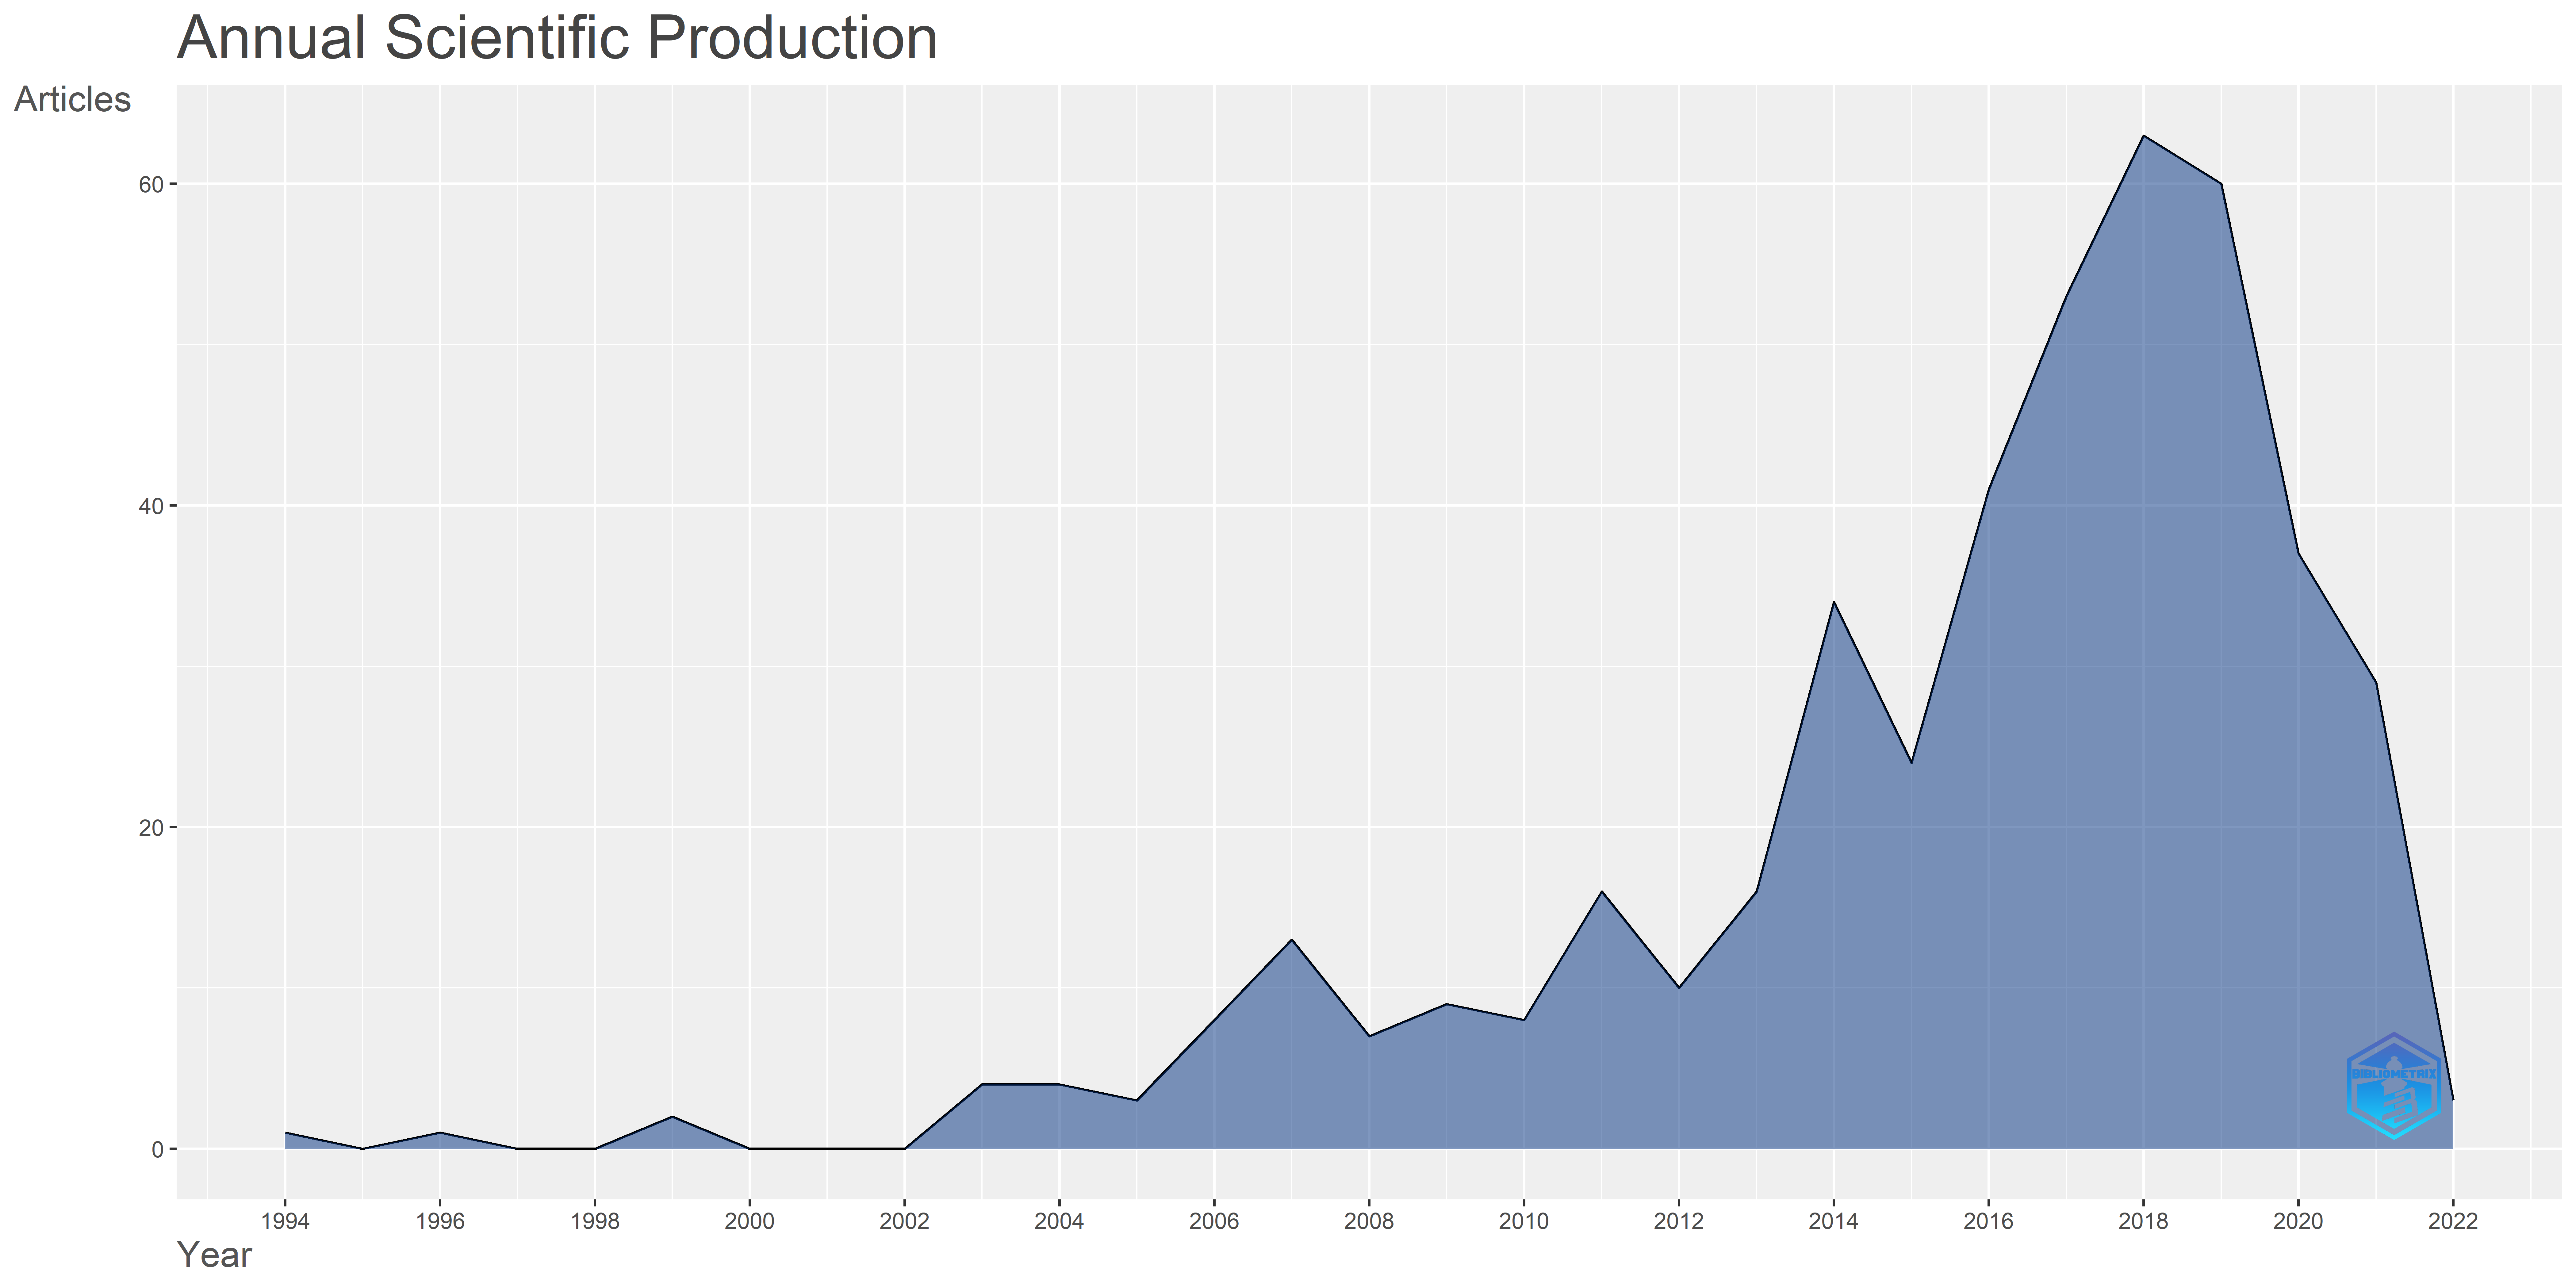
\includegraphics[width=1\textwidth]{experiments/Tatianafp/AnaliseBibliometrica/AnnualScientificProduction.png}
    \caption{Evolução da produção científica no \dataset\  NewsRec@Tatianafp.}
    \label{fig:evol_anual_NewsRec_Tatianafp}
\end{figure}

O \textit{Annual Growth Rate} encontrado no \dataset\  NewsRec@Tatianafp é de 5.12\%, consideravelmente maior que a taxa de crescimento anual da publicação científica mundial, de cerca de 3.3\%.

Ao observarmos a diferença entre a quantidade de publicações entre os anos de 2014 e 2018, os dois picos de crescimento, nota-se que o número quase que duplica. Isso indica que provavelmente ocorrera uma descoberta importante no ano de 2018, o que incentivou a pesquisa sobre o tema de sistemas de recomendação de notícias. No entanto, houve uma queda na produção científica nos anos posteriores ao ano de 2018, o motivo para tal ainda necessita de maiores investigações.  

\subsection{Análise da Colaboração entre Países}

Ao explorar o \dataset\  NewsRec@Tatianafp com o auxílio da ferramenta Bibliometrix, também é possível analisar como ocorre a colaboração entre os diversos países na produção científica relacionada ao tema de sistemas de recomendação de notícias. A imagem \ref{fig:country_collab_NewsRec_Tatianafp} retrata o gráfico que fora obtido. 

\begin{figure}
    \centering
    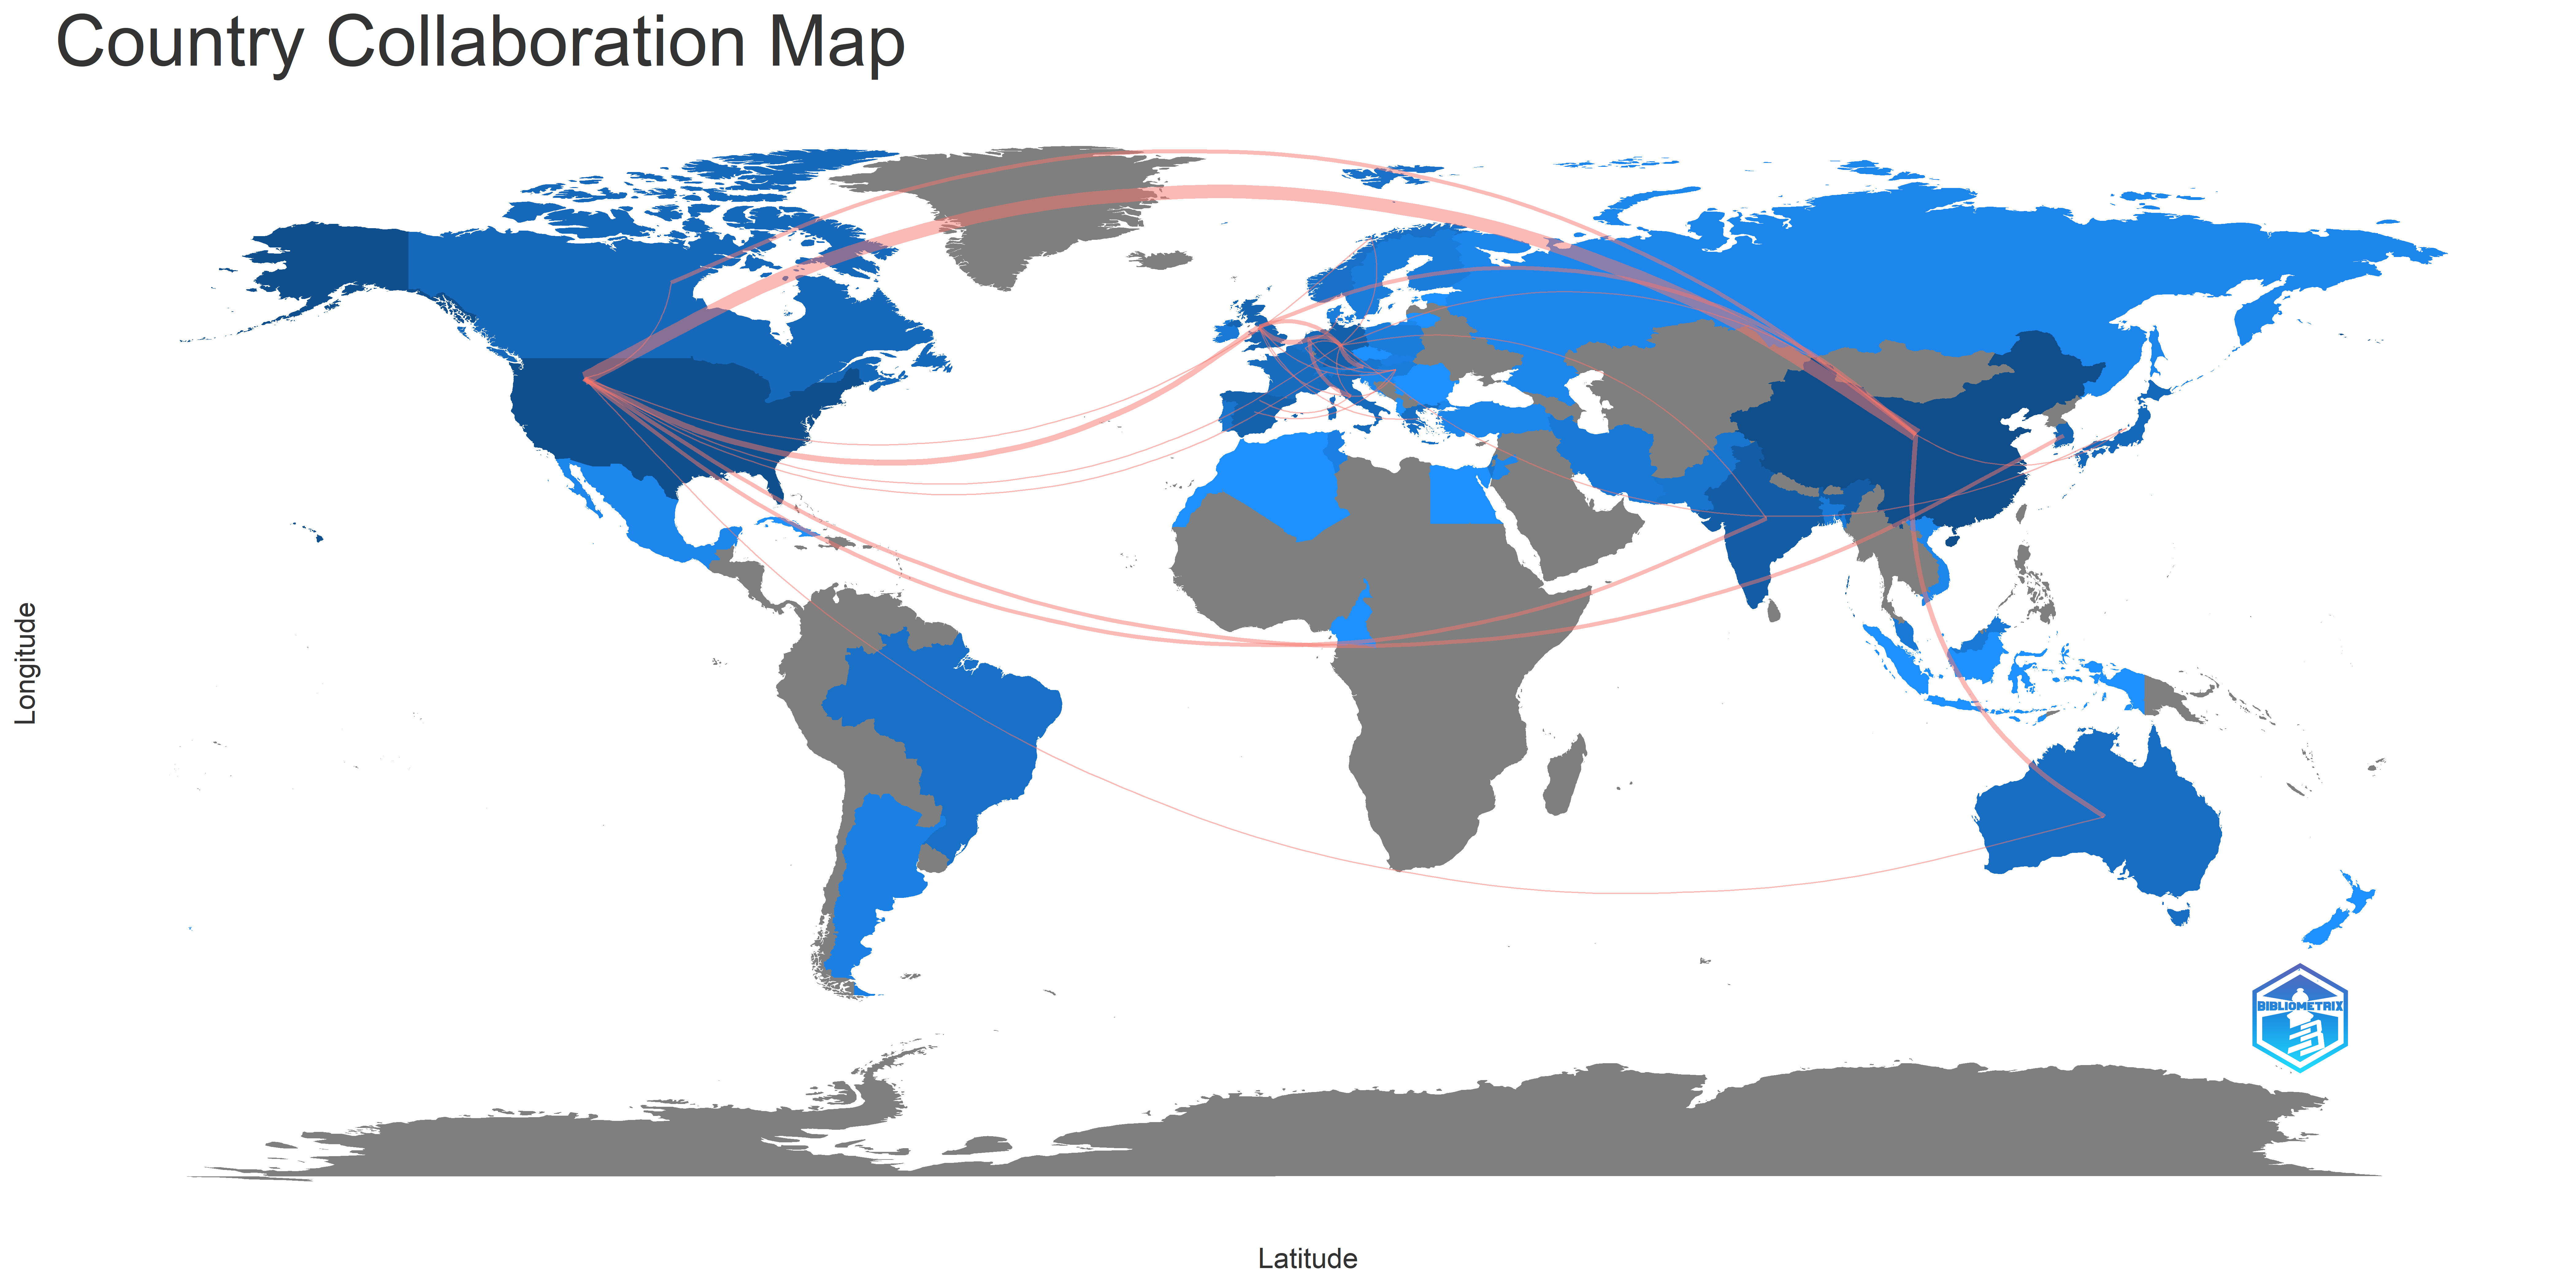
\includegraphics[width=1\textwidth]{experiments/Tatianafp/AnaliseBibliometrica/CountryCollaborationMap.png}
    \caption{Colaboração entre países segundo o \dataset\  NewsRec@Tatianafp.}
    \label{fig:country_collab_NewsRec_Tatianafp}
\end{figure}

Ao analisar a imagem \ref{fig:country_collab_NewsRec_Tatianafp} nota-se uma alta colaboração entre os Estados Unidos e China, acompanhados por colaborações com países da Europa e mais alguns países da Ásia como Índia, Japão e Coréia do Sul. Também se tem um volume considerável de contribuições com a Austrális e com o Canadá. Apesar de estar destacado no mapa, o Brasil não tem suas colaborações representadas pelas linhas que ligam os países. Isso ocorre devido ao seu número pequeno de colaborações, se resumindo a apenas três, conforme apresentado na tabela \ref{tab:Brasil_collab_Tatianafp}

\begin{table}[htp]
    \centering
\footnotesize
\csvreader[tabular = |r|l|l|r|r|,
separator=semicolon,
filter={\value{csvrow}<25}
%,filter not strcmp={\csvcolii}{},
, table head = \hline\hline \# & País  & País  & Frequência\\ \hline\hline,
table foot = \hline\hline
]{experiments/Tatianafp/World_Collaboration_Map.csv}{Document=\paper, DOI=\doi}{ \thecsvrow & {\tiny\paper} & {\tiny \doi} & \csvcoliii & \csvcoliv}

    \caption{Colaborações entre o Brasil e demais países no \dataset\ NewsRec@Tatianafp.}
    \label{tab:Brasil_collab_Tatianafp}
\end{table}



